\chapter{Colorization}
\label{chapterlabel3}

Colorization is the process of adding plausible colors to monochrome images, it is a highly uncertain problem that has not a unique solution. In the context of this master project, we are interested in anime-style sketch colorization, a few distinctive characteristics includes:

\begin{itemize}
    \item Unlike grayscale image input, its input is a binary sketch image.
    \item Unlike realistic image colorization, the output is heavily style-oriented, has less well-defined details, and therefore comparably nondeterministic nature.
    \item Unlike many colorization researches, the task of filling missing regions is not assessed. The full sketch image is provided without cropping.
    \item It is relatively difficult to find a dataset that contains large amount of high quality pairs of sketch and colorized anime image, because artists often do not include it when uploading to the internet.
\end{itemize}


\section{Approaches \& Methods}
Anime-style sketch colorization is a sub-field in image-to-image translation task. It is a difficult problem because there are infinite number of ways to produce feasible results, therefore color strokes are often given as additional input to hint the model to output in a certain style (user-guided colorization). There are many attempts to this problem and I will introduce them in the following paragraphs.

Traditional computer assisted colorization uses an algorithmic approach. Typically, the user first crops the region that he/she wants to color, then apply a color scheme from a palette, finally the computer will run an algorithm to perform colorization. A popular approach is to minimize the difference between a pixel's color and its weighted average of neighbouring pixels' colors.\cite{levinColorizationUsingOptimizationb} The intuitive is neighboring pixels with similar intensity should have similar colors. This method generates high quality results, but it is time consuming because it requires detailed color input and manual cropping. Follow up researches attempted to reduce the effort via learning-based methods, such as interpolation of user-drawn scribbles using boosting \cite{liScribbleBoostAddingClassification2008} or manifold learning \cite{chenManifoldPreservingEdit2012}; and determine the importance of image feature automatically using neural network \cite{endoDeepPropExtractingDeep2016}.



\begin{figure}
    \centering
    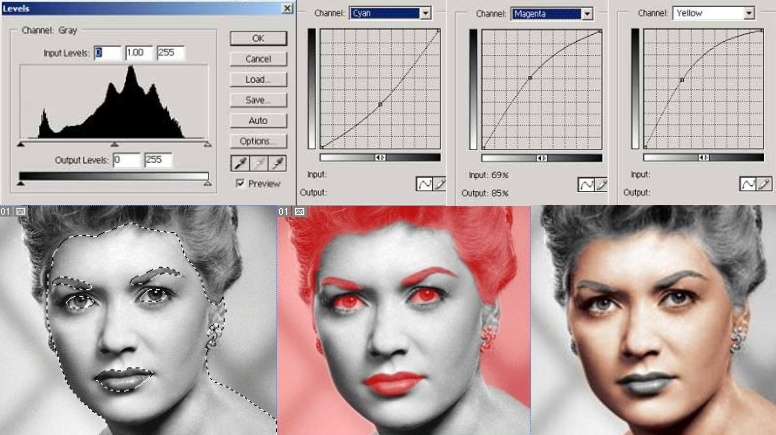
\includegraphics[width=0.75\textwidth]{images/colorization/computer_assisted_colorization.jpg}
    \caption{Example interface for traditional computer assisted algorithmic colorization. Top shows an interface for selecting a color; bottom-left and bottom-middle show interfaces for selecting a region; and bottom-right shows the resulting image.\cite{ColorizeBlackWhite}}
    \label{fig:computer_assisted_colorization}
\end{figure}

While these methods introduced remarkable improvements, image colorization remains a time-consuming task. In addition, traditional methods often make use of intensity information which does not presents in anime sketches, which made them unsuitable. In recent years, machine learning based methods started to gain popularity as availability of computing resource increases. The milestone work of Pix2pix\cite{isolaImagetoImageTranslationConditional2018} demonstrated a simple yet general architecture for image-to-image translation task. It outperforms vanilla CNN by a large margin (see figure \ref{colorization_cnn}) However, directly apply Pix2pix model will result in artifacts such as \textit{color bleeding}\footnote{Color overflows boundaries defined by sketches.} and \textit{dirtiness}\footnote{Abrupt smoky color patches that are not defined by the sketches.}, these result in style inconsistency and unpleasing colorization (see figure \ref{fig:colorization_pix2pix}). 

\begin{figure}
    \centering
    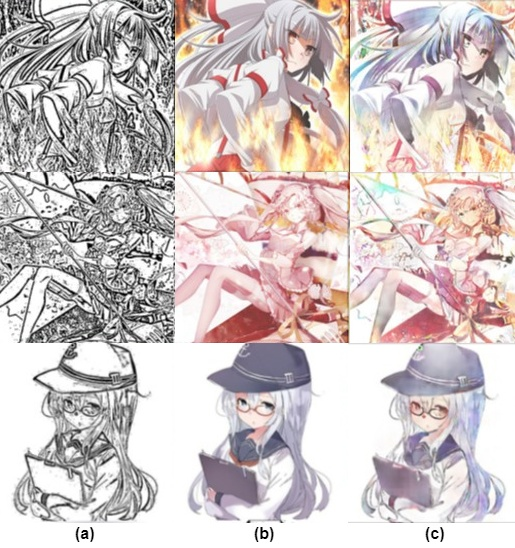
\includegraphics[width=0.75\textwidth]{images/colorization/cnn.jpg}
    \caption{Vanilla CNN output for anime sketch colorization. Column (a) is the input sketches; column (b) is the target image; and column (c) is the output image.\cite{fransOutlineColorizationTandem2017} We can see that the output suffers from a number of obvious issues, such as fading colors, obvious convolutional artifacts, and messy colors. It is far from visually pleasing.} 
    \label{fig:colorization_cnn}
\end{figure}


\begin{figure}
    \centering
    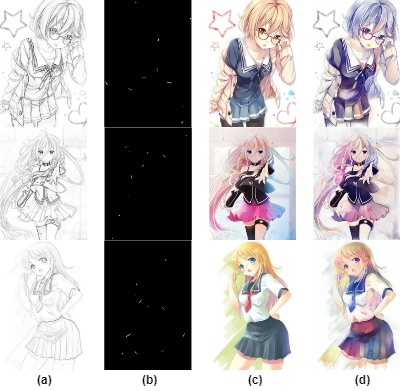
\includegraphics[width=0.75\textwidth]{images/colorization/pix2pix.jpg}
    \caption{Vanilla Pix2pix output for anime sketch colorization. Column (a) is the input sketches; column (b) is the color hint; column (c) is the target image; and column (d) is the output image.\cite{steinsDeepLearningProject2022} The coloring are reasonable but suffer from artifacts such as color bleeding and has a certain degree of dirtiness. For example, the colors are different in each stripe of the skirt and random smoky regions are generated.} 
    \label{fig:colorization_pix2pix}
\end{figure}


PetalicaPaint\cite{PetalicaPaint} used a doubly linked deep U-Net architecture to address style inconsistency problem, by having a deeper network, the model is able to capture the general distribution and keep it consistent. However, it's style varies on loss function hyper-parameters which means each model can only paint with one style (see figure \ref{fig:colorization_petalica}).


\begin{figure}
    \centering
    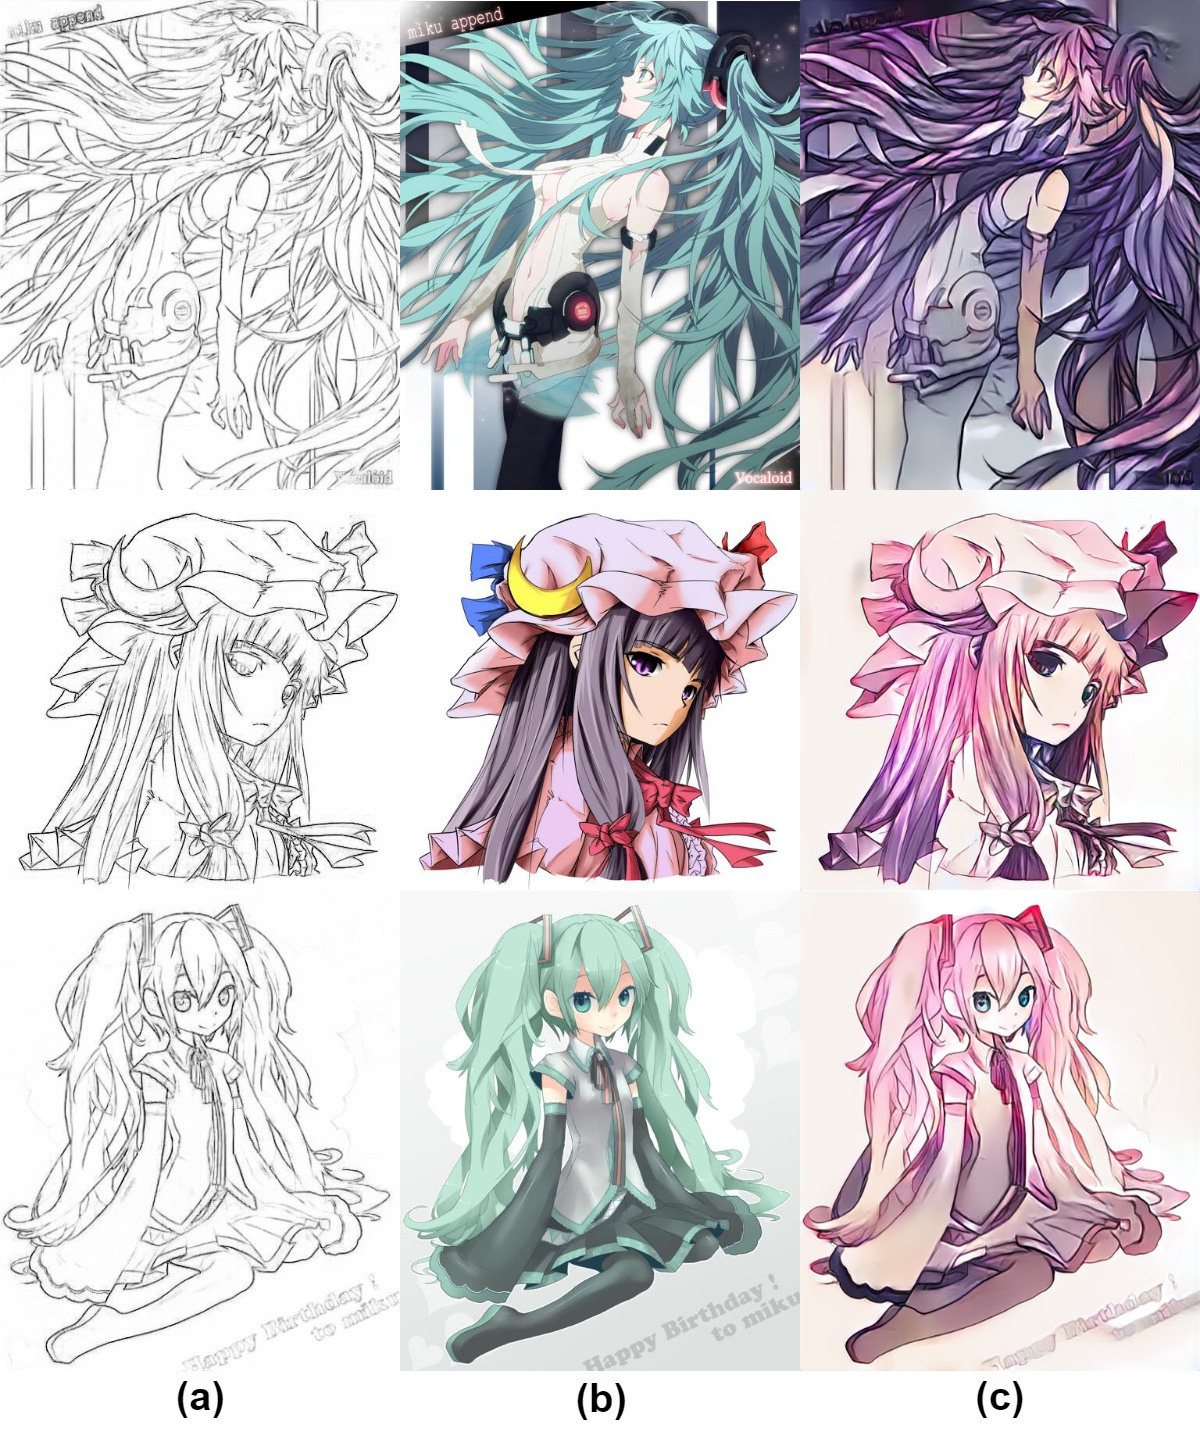
\includegraphics[width=0.75\textwidth]{images/colorization/petalica.jpg}
    \caption{Petalica Paint output for anime sketch colorization, painted with \textit{Canna\protect\footnotemark}  style. Column (a) is the input sketches; column (b) is the target image; and column (c) is the output image.\cite{steinsDeepLearningProject2022} The coloring showed consistency across different region with clean and pleasible coloring, however, there is little artistic texture and global shading presents in the colored image.} 
    \label{fig:colorization_petalica}
\end{figure}

\footnotetext{The name of the style given to a particular model by the author.}

Although the result is much more pleasing, it is still not as vivid as most colored image, two most obvious features missing are artistic texture and global shading. Artistic texture allows the model to have slightly different styles in different region of the image and global shading allows the model to draw sensible shadows and highlights. Fortunately, follow up researches showed that we can obtain artistic texture by using content loss and obtain global shading simply by using a deeper U-Net blocks.\cite{ciUserGuidedDeepAnime2018} (See figure \ref{fig:colorization_alacgan})

\begin{figure}
    \centering
    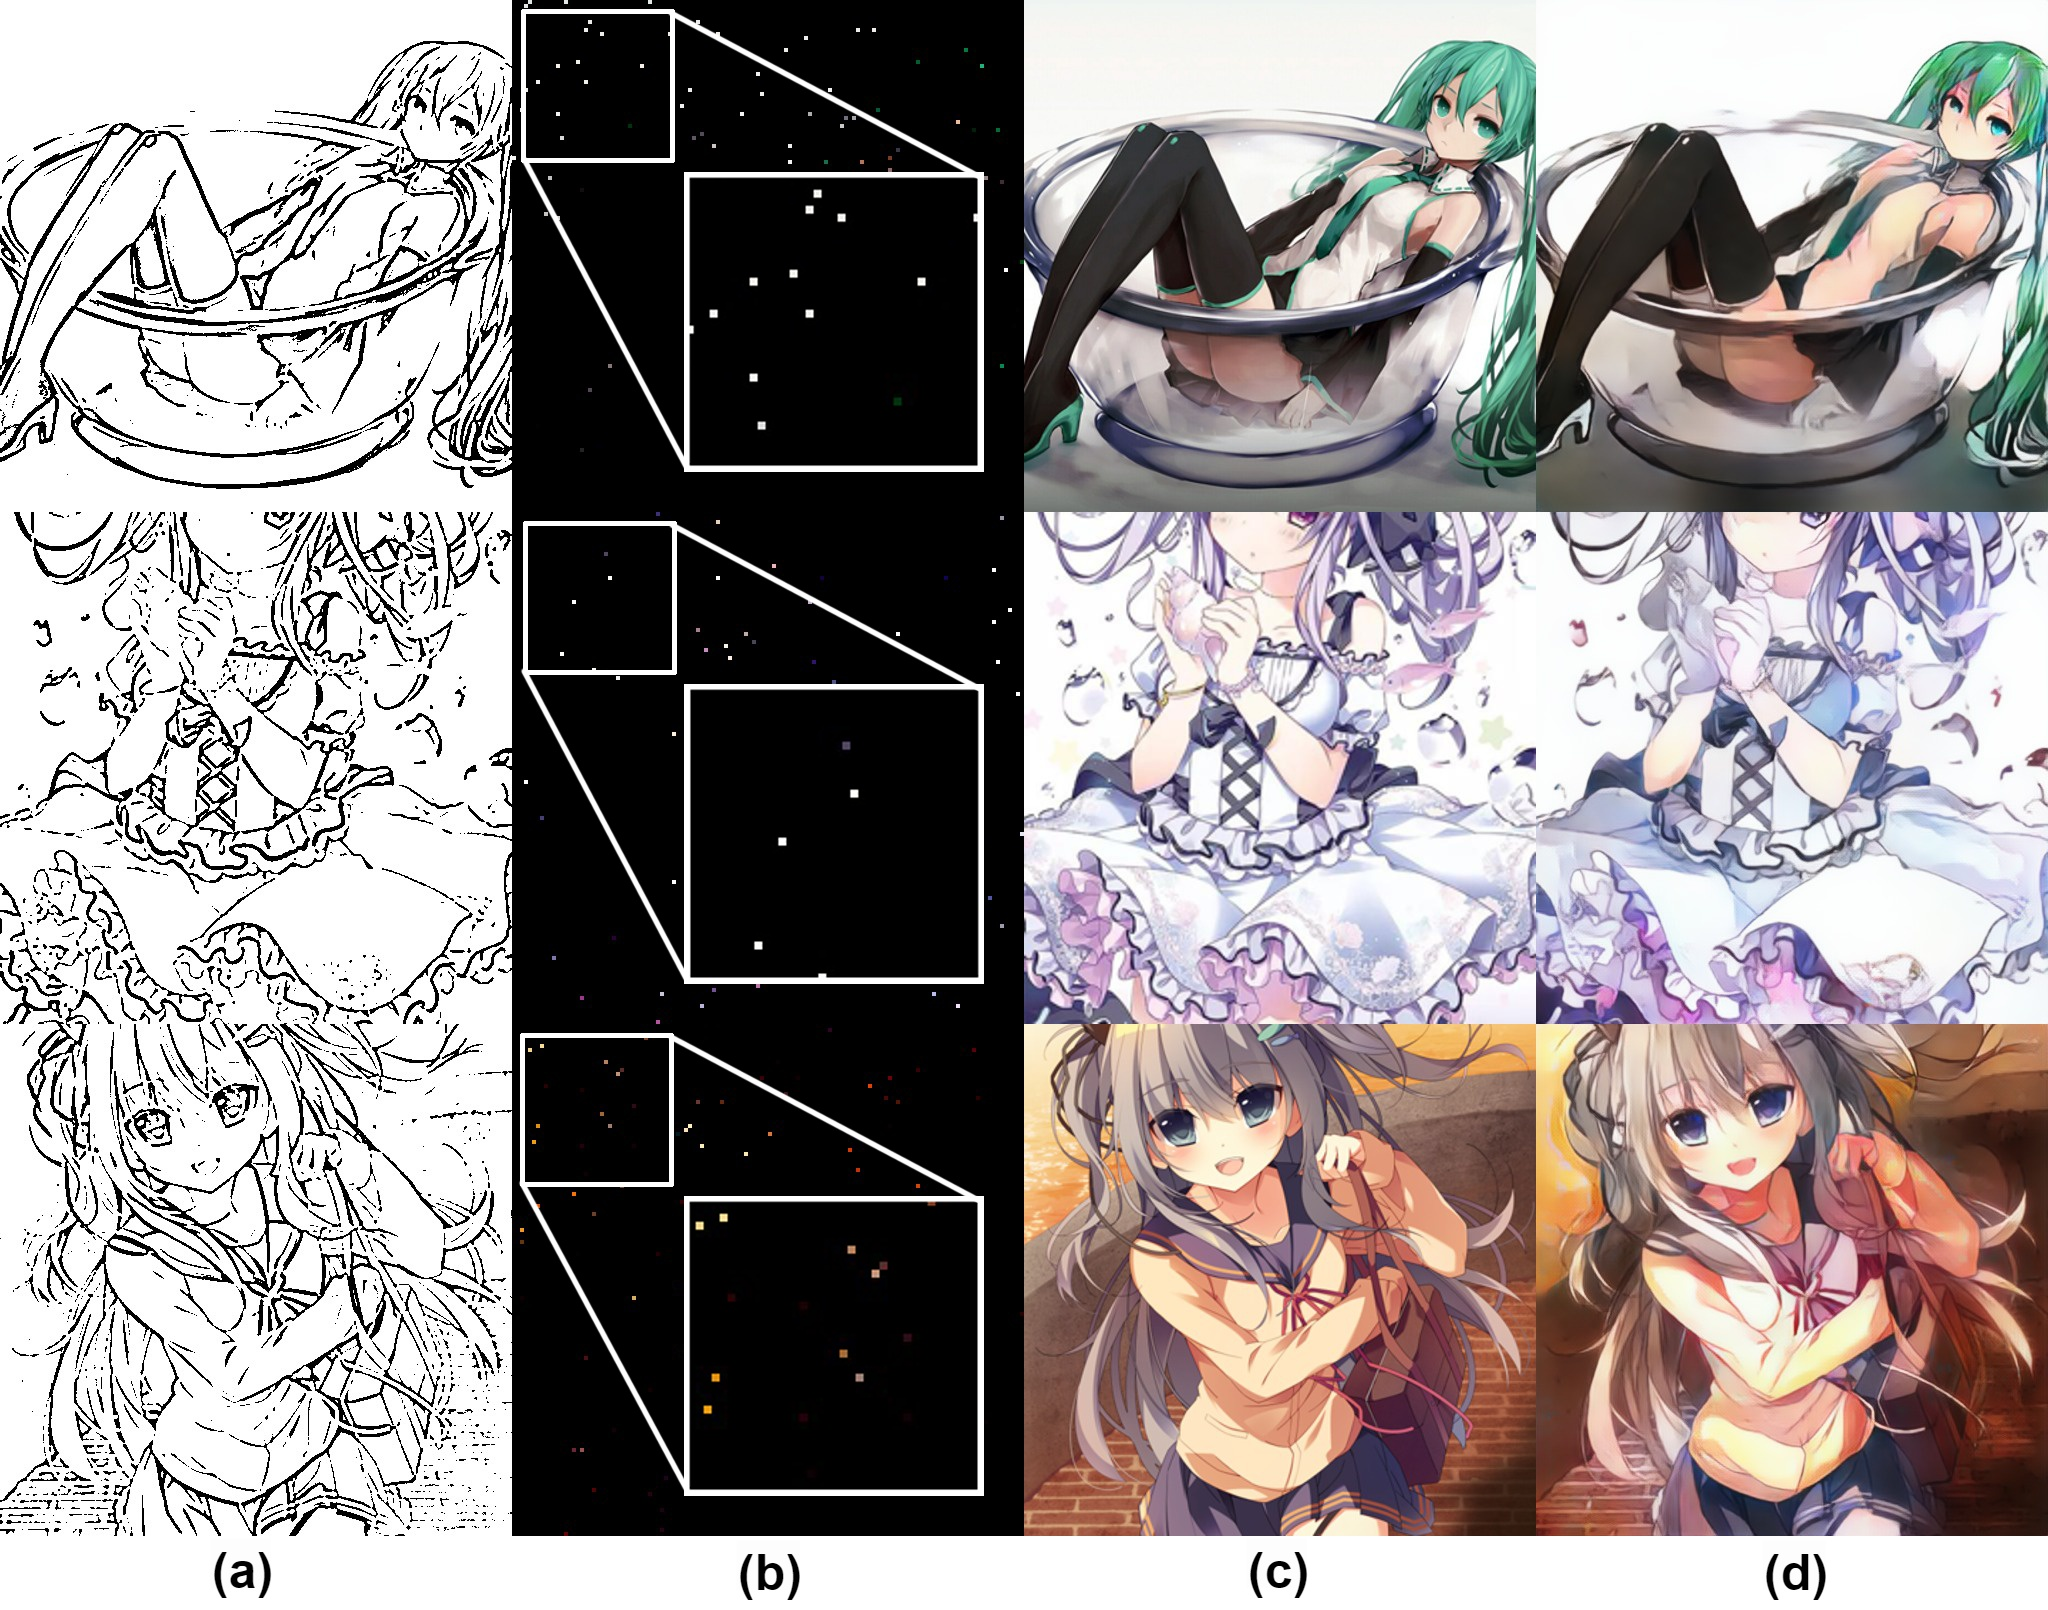
\includegraphics[width=0.85\textwidth]{images/colorization/alacgan.jpg}
    \caption{AlacGAN output for anime sketch colorization. Column (a) is the input sketches; column (b) is the color hint; column (c) is the target image; and column (d) is the output image. We can observe that the present of global shading and diverse artistic textures result in a much more vivid output.} 
    \label{fig:colorization_alacgan}
\end{figure}

\section{Design \& Implementation}
XDoG + U-Net + deep decoder + ResNeXt block + vgg feature layer + color hint + content loss + l2 loss

%The input to the model is binary anime sketches, they are synthesized from real anime images with XDoG boundary detection filter\cite{winnemollerXDoGEXtendedDifferenceofGaussians2012}.

\begin{figure}
    \centering
    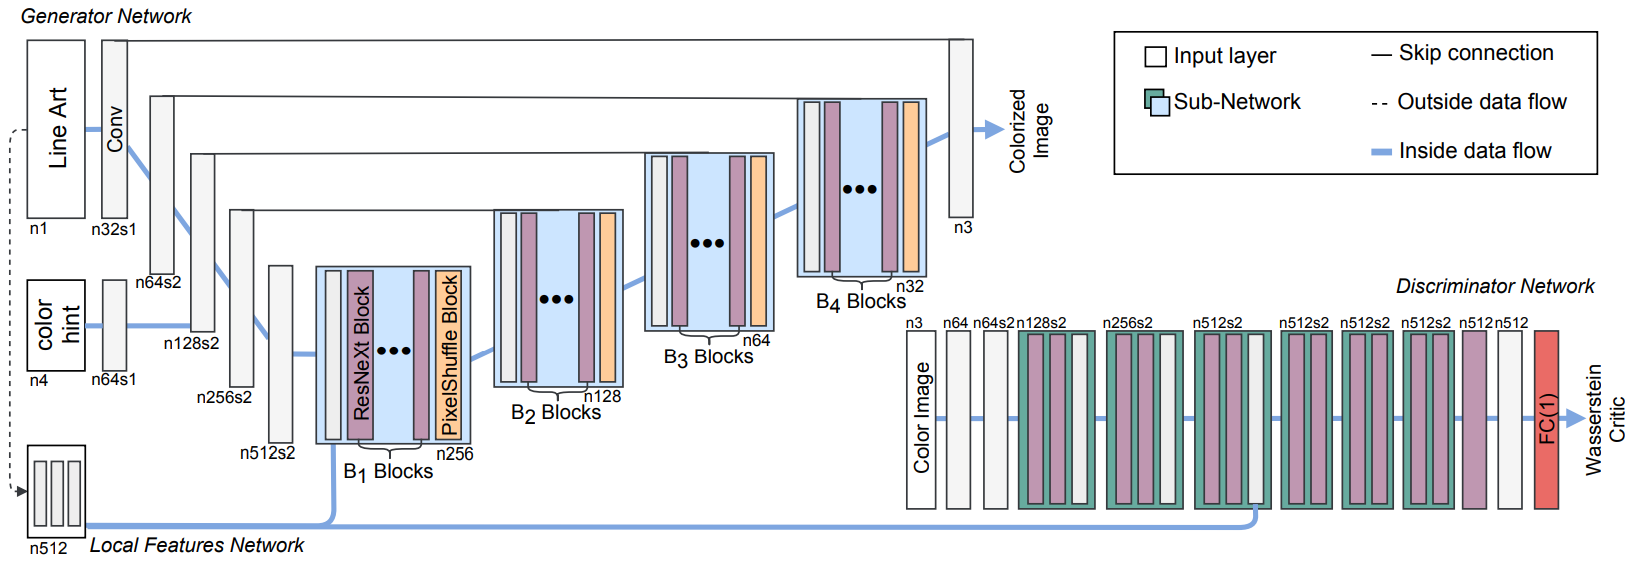
\includegraphics[width=1.0\textwidth]{images/colorization/alacgan_arch.png}
    \caption{Architecture of Generator and Discriminator Network with corresponding number of feature maps (n) and stride (s) indicated for each convolution block.} 
    \label{fig:alacgan_arch}
\end{figure}

\section{Results \& Analysis}

